\chapter{FM-радио для хипстера}

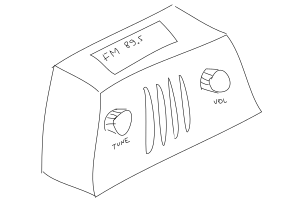
\includegraphics{sketches/fm-radio}

% Количество концептов (сколько новых понятий вводим)
% _ _ _ _
%
% Глубина подачи концептов (насколько подробно объясняются)
% _ _ _ _
%
% Необходимость концептов (насколько обязательны концепты для проекта)
% _ _ _ _

Итак, наконец-то, к первому проекту! Начнём с чего-нибудь простого, но в то же время условно-полезного. В качестве такого устройства я выбрал настольное FM-радио с классическим управлением двумя поворотными ручками и ЖК-дисплеем для отображения информации.

Вроде бы уже давно настала эра цифрового радио и стриминг-сервисов, но всё равно, порой не хватает аскетичного приёмника, который можно включить одним движением без поиска нужной иконки, без сопряжения с беспроводными колонками, без всей этой суеты. А с учётом того, что вы можете сделать уникальный корпус, можно быть уверенным, что самоделка займёт своё место в интерьере. Поехали!

% TODO: перечислить фактические знания

В этой главе вы узнаете, как работать с текстовым ЖК-экраном, энкодером и чипом FM-приёмника; что такое шина I²C; как устроено воспроизведение звука; и многое другое.

\section{Необходимое железо}

% TODO: лист картинок

\begin{itemize}
  \item Ардуино-совместимая плата: Arduino Uno, Iskra Uno, Iskra Nano или другая
  \item USB-кабель для прошивки и питания
  \item Модуль FM-приёмника на чипе TEA5767
  \item Усилитель аудиосигнала, например, на основе микросхемы PAM8403
  \item Динамик с импедансом 4 или 8 Ом
  \item Потенциометр для управления громкостью
  \item Поворотный энкодер для переключения радиостанций
  \item Текстовый ЖК-экран
  \item Провода
  \item Беспаечная макетка (breadboard) для прототипа
\end{itemize}

Опционально:

\begin{itemize}
  \item Модуль пауэр-банк для автономной работы
  \item Тумблер для включения / выключения
  \item Макетка под пайку для финальной сборки
  \item Гнездо под штекер 3.5 мм с клеммником
\end{itemize}

\section{Как вещает радио}

Вы конечно знаете, что эфир радиостанций распространяется по-воздуху в виде неких магических невидимых волн. Где-то на радиостанции стоят антенны и оборудование, которые перепаковывают звуковой сигнал в электромагнитный и вещают его во все стороны. Если мы хотим услышать, что происходит в эфире, мы должны этот радиосигнал поймать, распаковать обратно в звуковой вид и отправить на динамик.

Но как это сделать? Нужно разобраться, как устроен FM-сигнал. Итак, по воздуху можно распространять радиоволны. У каждой радиоволны есть \emph{частота}. Эта характеристика говорит о том, сколько раз в секунду встречается пик этой волны. Например, частота в 89.5 мегагерц означает, что пик будет встречаться 89.5 миллионов раз в секунду. Часто, не правда
ли? Волны разной частоты можно отделять друг от друга, немного корректируя схему приёмника. Поэтому, на частоте 89.5 МГц сигнал может транслировать одна радиостанция, а на частоте 90.0 Мгц уже другая. При этом они не будут мешать вашему домашнему Wi-Fi, потому что он вовсе работает на частоте около 2.4 или 5 ГГц.

\begin{figure}
  \centering
  % TODO: перерисовать через Matplotlib + xkcd, показать суперпозицию
  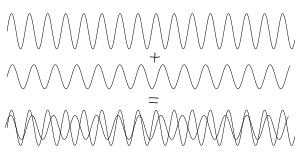
\includegraphics{sketches/wave-lengths}
  \caption{Волны разной частоты формируют эфир}
\end{figure}

\begin{Note}
  А вот сигналы, посылаемые волнами схожих частот очень даже мешают друг
  другу и это серьёзная проблема современных городов, которая заставляет
  занимать для разных целей всё новые и новые диапазоны частот. Диапазон
  частот называется полосой, а разрешают или запрещают их использование
  разные дядьки в министерствах. Но это уже другая история.
\end{Note}

Хорошо, с частотой несущей волны разобрались. Но как с помощью неё передать информацию? В нашем случае звуковой ряд. Тут в дело вступает трюк, который называется модуляцией. Кстати, «FM» означает «фазовая модуляция». Суть трюка заключается в том, чтобы менять фазу несущей частоты в соответствии с тем, какой звуковой сигнал нужно передать: несущую волну сжимают и растягивают как гармошку, чтобы дополнить полезной информацией. Драматично на частоту несущей волны это не влияет, т.к. силы не равны: килогерцы звуковой волны против гигагерц несущей.

% TODO "Грубая иллюстрация принципа фазовой модуляции"
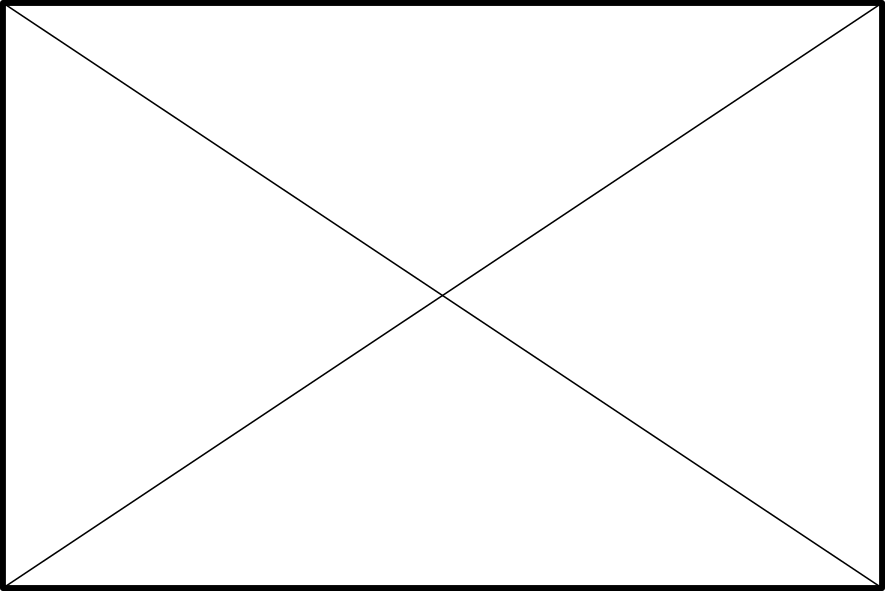
\includegraphics{TODO.png}

Вроде бы разобрались. Так как имея на руках несколько проводов и пару резисторов, поймать волну и расшифровать её? Можно собрать внушительную схему из отдельных компонентов, как делали наши отцы и деды. Но время идёт и для многих типовых задач давно существуют готовые \emph{микросхемы} (также известные как \emph{чипы}), которые скрывают всю схему под крохотным пластиковым корпусом, а для своей работы требуют минимум дополнить компонентов.

\section{Знакомьтесь, TEA5767!}

Чипом, предназначенным специально для приёма и демодуляции FM-радио является дешёвый и популярный TEA5767 от компании Philips. В своём оригинальном виде он предназначен для ширпотребной и миниатюрной электроники, которую производят промышленным образом. Поэтому он настолько мал, что вам, как мейкеру, было бы крайне неудобно работать с ним, если речь идёт о ручной сборке одного или нескольких устройств. К тому же для своей работы он требует несколько дополнителльных компонентов вроде кварцевого резонатора.

Ленивое и алчное человечество не остановилось на создании миниатюрных чипов. Специально для вас, мейкеры, некоторые компании берут такие маленькие чипы, увеличивают их в размерах, распаивая на печатной плате вместе с необходимым обвесом и продают втридорога \textbar emoji\_smiling\_imp\textbar{} Но ведь девайс собранный своими руками бесценен, не так ли?!

Для нашего радио нам понадобится один из таких готовых модулей.

\begin{figure}
  \centering
  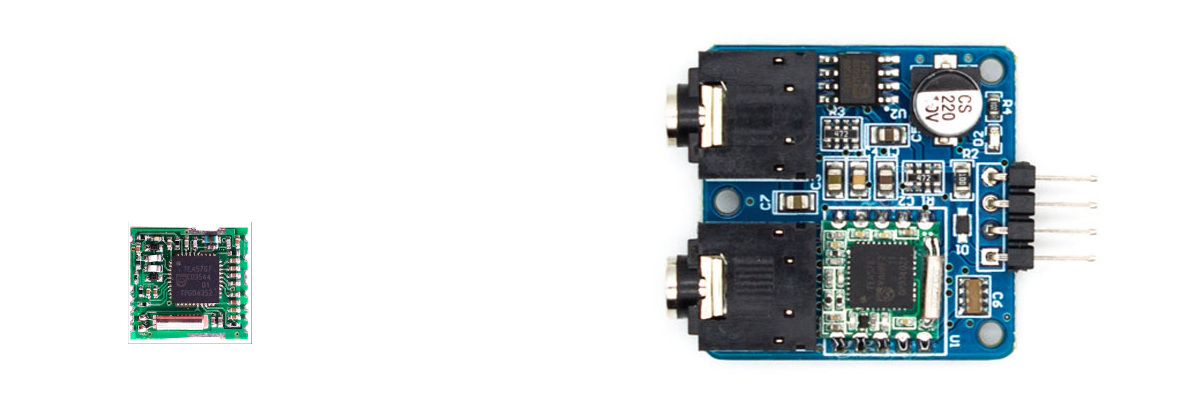
\includegraphics{TEA5767.jpg}
  \caption{Популярные вариации модуля на базе TEA5767}
\end{figure}

Что же он из себя представляет? Такой модуль является безголовым радио, которым нужно управлять не кнопками и ручками, как на готовой аудио-системе, а командами с конроллера. Контроллером может запросто выступать ваша Arduino-совместимая плата. Контроллер может попросить настроиться на определённую частоту, начать промотку каналов в одну или другую сторону, запросить уровень сигнала, а в качестве выхода модуль на TEA5767 выдаёт аудиосигнал.

\begin{figure}
  \centering
  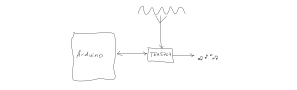
\includegraphics{sketches/fm-receiver-diagram}
  \caption{Диаграмма включения модуля FM-приёмника}
\end{figure}

Давайте теперь разберёмся, как именно общаться с модулем. Такой модуль с точки зрения взаймодействия несколько сложнее, чем светодиод или кнопка: коммуникация с ним строится через так называемый интерфейс I²C. Пусть вас это не пугает: благодаря тому, что для популярных модулей уже созданы библиотеки, работа с ними становится вполне тривиальной.

\begin{Note}
  % TODO: emoji
  Я надеюсь, что вы не сильно устали, потому что всё написанное выше и под следующим заголовком на деле не нужно для того, чтобы сделать радио \textbar emoji\_smile\textbar. Но этими знаниями можно вполне хвастануть за бокалом пива. Сразу после, обещаю, мы приступим к сборке.
\end{Note}

\section{Интерфейс I²C}
\label{I2C}

I²C, он же IIC, он же «айтуси», он же «идвацэ», он же TWI — крайне распространённый интерфейс в мире цифровой микроэлектроники для подключения устройств. Так если в своём компьютере вы скорее всего найдёте интерфейсы USB, Display Port и Ethernet, то на конроллере вы найдёте другой набор интерфейсов: UART, SPI и I²C. Они пусть менее гибкие и богатые на возможности, но гораздо более простые и непритязательные к вычислительным ресурсам.

В случае с I²C всегда одно из устройств выступает ведущим (master), а другое ведомым (slave). Ведущим как правило является контроллер Arduino, а ведомым — модуль или чип. Обмен данными между устройствами по I²C осуществляется по двум сигнальным линиям, т.е. проводам:

% TODO: definition list

SDA Линия данных. Высокий сигнал вроде 3.3 или 5 вольт (зависит от родного напряжения участников) означает передачу бита-единички, низкий сигнал 0 вольт означает передачу бита-нолика. В какую сторону передаются данные в данный конкретный момент зависит от ситуации, а вернее от \emph{протокола}, на который негласно договорились участники коммуникации.

SCL Линия тактирования. Очередной бит считается переданным, после того как линия сначала получает высокий сигнал, а затем низкий. Сигналом на SCL всегда управляет мастер, вне зависимости от направления передачи данных. Так он задаёт скорость коммуникации. Задача ведомого устройства — поспевать.

\begin{figure}
  \centering
  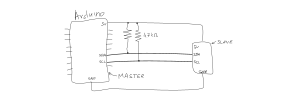
\includegraphics{sketches/i2c-single}
  \caption{Типовой пример подключения одного I²C-устройства}
\end{figure}

I²C — это шина (bus). Под этим понимается, что на одной и той же паре линий SDA/SCL может быть подключено множество разных устройств. Если быть точным, до 127 ведомых устройств.\footnote{Если быть совсем точным, то расширенный стандарт позволяет подключить в теории и до 32 тысяч устройств, но это совсем экзотика. В мире хобби-электроники не встречал.} При этом, у любого устройства на шине, будь оно единственным или нет, есть собственный адрес, по которому ведущий обращается именно к нему.

\begin{figure}
  \centering
  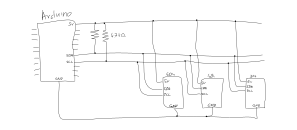
\includegraphics{sketches/i2c-multiple}
  \caption{Типовой пример подключения нескольких I²C-устройств}
\end{figure}

С этой точки зрения, шина I²C похожа на роту модулей построенную на плацу, где командование ведёт офицер-контроллер. Все слышат всё, но говорит только один:

— Рядовой 60h!\\
— Здесь!\\
— Частоту радио на 89.5 МГц установить!\\
— Есть!\\
— Частоту радио на 1000 МГц установить!\\
— Никак нет!\\
— Уровень сигнала сообщить!\\
— Двенадцать!

Адрес конкретного модуля обычно жёстко задаётся на производстве, на уровне микросхемы. Например, адрес TEA5767 — 60 в шестнадцатиричной системе, что обычно записывают как \texttt{60h} или \texttt{0x60}.  Детали протокола также определяются разработчиками модуля, а все его подробности всегда подробно описаны в даташите от производителя.

К счастью, для многих популярных модулей уже существуют высокоуровневые библиотеки-обёртки, которые вовсе снимают необходимость в том, чтобы разбираться в тонкостях их протоколов. Это справедливо и для нашего FM-приёмника. Так что мы уже готовы действовать. Вперёд!

\section{Подключаем FM-ресивер}

Будем строить девайс в несколько этапов. Сначала попробуем заставить выдавать наше радио хоть что-то. Для этого соберите схему, как показано на рисунке \ref{fig:tea5767-wiring}.

\begin{figure}
  \centering
  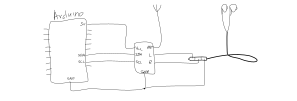
\includegraphics{sketches/tea5767-wiring}
  \caption{Схема подключения модуля TEA5767 к Arduino}
  \label{fig:tea5767-wiring}
\end{figure}

Для сборки используйте макетные провода и бредборд. Где возможно, не соединяйте пока всё намертво паяльником: нам ещё предстоит дополнять схему. И в конце концов, нужно предварительно убедиться, что всё работает.

В зависимости от выбранной модели FM-модуля вам может понадобиться припаять к модулю ножки-штырьки. Если на борту модуля нет разъёма 3.5 мм для непосредственного подключения наушников, вы можете использовать TRS-гнездо с клеммником, чтобы быстро адаптировать пины L, R и GND на модуле в стандартный аудиоразъём (рис. \ref{fig:trs-35-mm}).

\begin{figure}
  \centering
  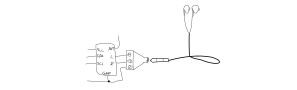
\includegraphics{sketches/trs-35-mm}
  \caption{Подключение наушников через клеммный разъём 3.5 мм}
  \label{fig:trs-35-mm}
\end{figure}

А нельзя ли сразу подключить динамик, который мы планируем использовать в финальном устройстве? Нет, пока нет. Дело в том, что модуль выдаёт слишком слабый аудиосигнал, который не сможет качать мембрану крупного динамика. Да и низкий импеданс динамика или больших наушников может спровоцировать токи, на которые FM-модуль просто не рассчитан, и вывести его из строя. Но на маленькие наушники-капельки выхода модуля вполне хватит.\footnote{Если у вас голый зелёный модуль, состоящий из чипа и металлической капсулы с кварцевым резонатором, то по официальным документам и наушники-то он качать не сможет. Но на практике — может, хотя и тихо, в низком качестве.} Подойдёт также колонка с активным усилением, то есть та, у которой есть собственное питание и регулировка громкости.

В качестве антенны можно использовать ту, что была в комплекте с модулем, если она была, но в любом случае с этой задачей отлично справится простой кусок провода. Это даже лучше с эстетической точки зрения: его можно будет смотать и спрятать внутри корпуса. Главное, чтобы провод был правильной длины. Эта длина зависит от законов физики и длины радиоволн FM. Длина провода должна составлять ½ или ¼ от длины волны, что для 100 МГц, не вдаваясь в подробности, составляет 1426 или 713 мм соответственно. Отмерьте линейкой, отрежьте, зачистите с одной стороны и припаяйте к модулю.

Подключайте контроллер к компьютеру через USB: железо готово, сейчас будем программировать!

\section{Управляем ресивером с нодой tea576x-fm-radio-i2c}

% TODO: ниже шум или тишина?

Сейчас, если вы оденете наушники, скорее всего услышите шум в эфире. Нам нужно как-то заставить контроллер выставить частоту радиостанции. Самое время вспомнить какой-нибудь джингл с радио, чтобы опробовать модуль.  «— Мегаполис. Эйти найн, поинт файв, эф-эм. Зэ нэйшенл дэнс рэдио-стэйшн».

Для управления нашим модулем-приёмником в XOD уже реализована стандартная библиотека: \texttt{xod-dev/tea576x}. Найдите её в панели Project Browser и откройте, чтобы увидеть перечень доступных нод. Нас интересует \texttt{tea576x-fm-radio-i2c}. Это так называемая \emph{быстрая нода} (quickstart node), которой в одиночку будет достаточно для работы с большей частью функций железки. Создайте новый патч и разместите на нём эту ноду.

\begin{figure}
  \centering
  \includegraphics{projects/fm-radio--01-quickstart.png}
  \caption{Быстрая нода управления FM-приёмником}
\end{figure}

Обратите внимание, на пине \texttt{ADDR} уже установлено значение \texttt{60h}, что соответствует заводскому адресу модуля. Далее, пин \texttt{I2C} он принимает объект-шину. Если вы подключили всё, как было описано выше, этот пин трогать не нужно. Он необходим тогда, когда вы использовали дополнительный интерфейс контроллера, или вовсе решили его эмулировать на обычных цифровых пинах ввода-вывода.

% TODO: menu command

Далее, самое интересное, вход \texttt{FREQ}. На нём ожидается частота радио, заданная в мегагерцах. По умолчанию там \texttt{88.0}, но давайте установим его в частоту любимой радиостанции: \texttt{89.5}, например.  Готово! Загружаем программу: Deploy → Upload to Arduino → Upload. Одевайте наушники, если вы всё сделали правильно, вы услышите долгожданную музыку... или рекламу.

Время побаловаться, проверить как звучат разные станции. Перезаливать программу после каждой смены частоты не очень практично, поэтому лучше воспользоваться интерактивными возможностями XOD. Используйте ноду \texttt{tweak-number} из \texttt{xod/debug}: подключите её ко входу \texttt{FREQ}.

\begin{figure}
  \centering
  \includegraphics{projects/fm-radio--02-tweak-freq.png}
  \caption{Патч для интерактивной сессии с FM-приёмником}
\end{figure}

Загрузите программу снова в режиме со включённой отладкой. Теперь вы можете менять частоту в реальном времени и слышать, как меняется станция.

Прекрасно! Основа проекта готова. Время придать ему человеческий вид.

\section{Компоненты для плавной подстройки параметров}

Нашей целью является самодостаточное устройство. А каждый раз подключаться к компьютеру из XOD IDE, чтобы сменить станцию — не вариант. Нам нужен физический орган управления. На современных проигрывателях управление чаще реализовано на кнопках или вовсе в виде тач-интерфейса. Одна кнопка проматывает дапазон вперёд, другая — назад. Несколько кнопок отдают на то, чтобы запомнить радиостанции. Кнопочное управление — это вполне разумный вариант и мы могли бы поступить также. Но эстетика бы пострадала: мы делаем лаконичный радиоприёмник в стиле ретро, поэтому давайте используем какие-нибудь ручки-крутилки. Тем более, что они ни чуть не менее практичны.

С крутилками у нас есть два варианта: классический \emph{потенциометр}\footnote{Англ. «Potentiometer». Также его называют подстроечным резистором или переменным резистором.} или \emph{поворотный энкодер}.\footnote{Англ. «Rotary Encoder». Если контекст понятен, их ещё называют просто: энкодерами. Однако, «энкодер» — это широкое понятие и к ним ещё относятся, например, устройства для определения положения вала мотора.  Имейте это в виду при поиске информации.} Уверен, в быту вы имели дело с обоими. Ручка потенциометра свободно вращается от одного предела до другого, а используется он для примерного выставления параметра вроде температуры в морозилке или температуры обогревателя. Энкодер можно встретить на стиральной машине, микроволновке, или мультимедийной системе в машине. Это такие крутилки, у которых нет механических ограничений на угол поворота: их можно вращать бесконечно. Чаще всего рабочая окружность разбита на деления, и поворот ручки на одно такое деление сопровождается лёгкой фиксацией, чтобы она не могла зависнуть в промежуточном положении.

\begin{figure}
  \centering
  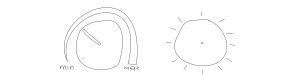
\includegraphics{sketches/pot-vs-encoder}
  \caption{Потенциометр против энкодера. Ручки обычно продают отдельно от самих сенсоров, чтобы можно было подобрать нужный размер и дизайн.}
\end{figure}

Потенциометр вполне подойдёт для регулировки громкости, но управлять с его помощью настройкой частоты будет не очень удобно. Смотрите сами, нам нужно выбирать частоту в диапазоне от 88.0 до 108.0 МГц с шагом 0.1. Всего получается 200 вариантов. При том что ручка типового потенциометры имеет ход в 270°, выходит, что соседние станции могут разделять всего пара градусов поворота. Понадобится ювелирная настройка. Да, в природе существуют многооборотные потенциометры. Но они довольно редки и дороги. Более практичный выбор — поворотный энкодер в котором одно деление будет соответствовать одному шагу на 0.1 МГц.

Решено. В этом проекте мы воспользуемся обоими сенсорами: потенциометром для громкости и энкодером для подстройки частоты.

\section{Поворотный энкодер}

Энкодеры бывают разных типов. Они бывают импульсными или абсолютными. Абсолютные всегда знают в каком положении находятся, а импульсные лишь генерируют последовательности импульсов определённой формы, которые должен интерпретировать контроллер и сам рассчитывать угол поворота. Также энкодеры различаются по количеству выходов (2, 3, 4 и т.д.) и внутреннему устройству (магнитные, оптические, ёмкостные). У всех есть определённые достоинства и недостатки. Для нас важна доступность, поэтому будем использовать самый популярный в DIY-мире и простой \emph{квадратурный} импульсный энкодер.

Принцип работы такого энкодера изображён на рисунке \ref{fig:quadrature-encoder}. У него есть два выхода — A и B — каждый из которых может принимать значение логической единицы или нуля. Переключение значений происходит со смещением в полфазы относительно друг друга, поэтому всего на выходе возможны четыре комбинации значений. Отсюда и название: квадратурный.

\begin{figure}
  \centering
  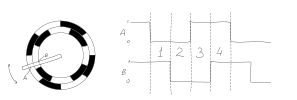
\includegraphics{sketches/quadrature-encoder-internals}
  \caption{Принцип работы импульсного квадратурного энкодера.}
  \label{fig:quadrature-encoder}
\end{figure}

Микроконтроллер должен фиксировать переключение сигналов A и B, и по изменению номера квадранта понимать, вращается ли ручка по часовой стрелке или против. В зависимости от этого можно либо наращивать внутренний виртуальный счётчик на один шаг, либо уменьшать.

Итак, чтобы задействовать наш энкодер для настройки радиоволны, подключите его к Arduino как показано на рисунке \ref{encoder-wiring}. В качестве пинов в нашем случае подойдут любые GPIO, которые не используются шиной I²C.\footnote{Для Arduino и Iskra Uno/Nano это A4 и A5; для Arduino и Iskra Leonardo/Neo/Micro это 2 и 3} Я выбрал пины 4 и 5.

\begin{figure}
  \centering
  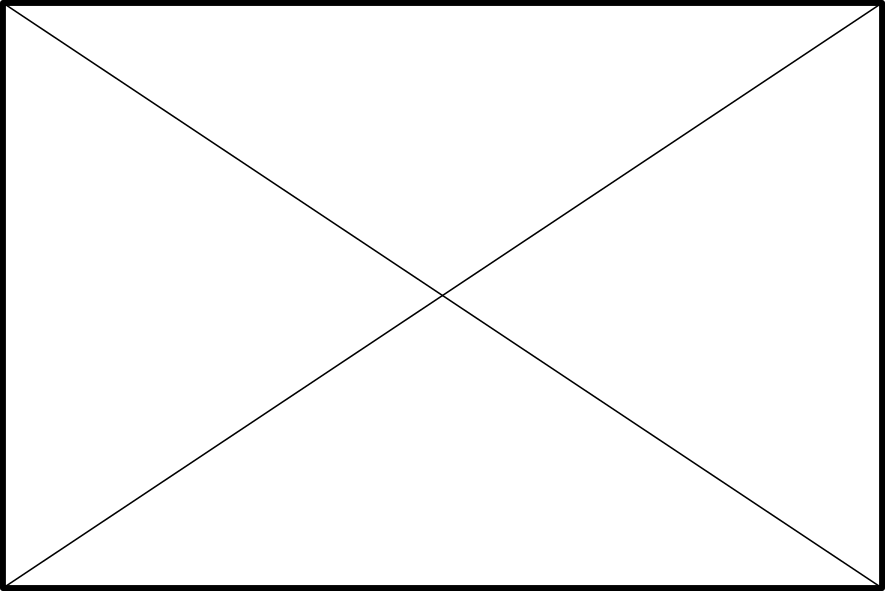
\includegraphics{TODO.png}
  \caption{Схема подключения энкодера к Arduino.}
  \label{encoder-wiring}
\end{figure}

В интернете можно встретить информацию о том, что подключать энкодер нужно строго к пинам, которые поддерживают так называемые аппаратные прерывания, но это обязательно только в тех устройствах, где переключения могут происходить очень быстро и есть шанс пропустить несколько переходов к очередной квадратуре из-за того, что контроллер был занят другой задачей. Например, это оправданно для подсчёта оборотов вала мотора. В нашем случае переключения происходят медленно, поэтому можно обойтись любыми цифровыми пинами.

\section{Ловим волну с нодами quad-encoder и count-bar}

Железо подключено, давайте программировать. Добавьте на свой патч ноду \texttt{quad-encoder} из \texttt{xod/common-hardware}. Её входы \texttt{PA} и \texttt{PB} определяют порты контроллера, куда подключен энкодер. Выставьте им значения \texttt{D4} и \texttt{D5} соответственно.

\begin{figure}
  \centering
  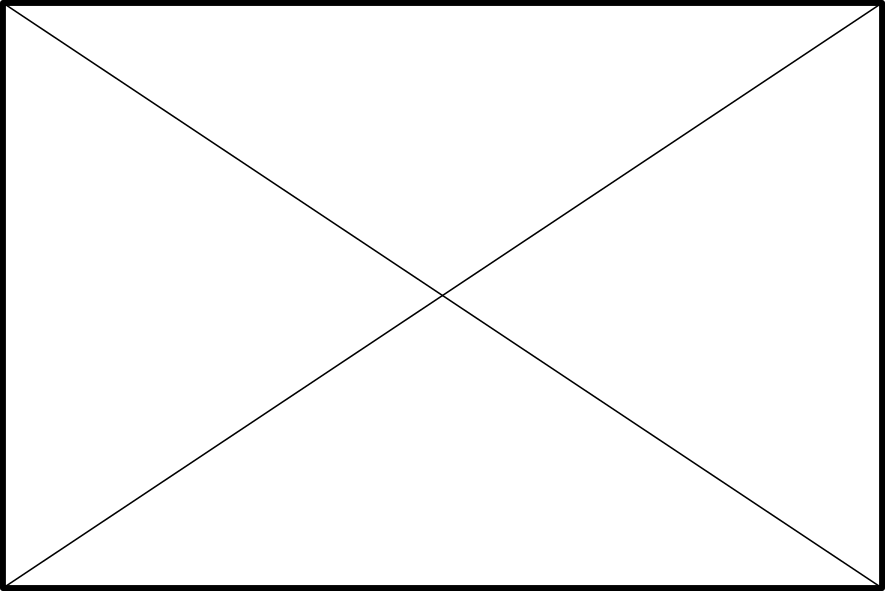
\includegraphics{TODO.png}
  \caption{Нода энкодера с отладочными вотчами на выходах.}
\end{figure}

У ноды есть два выхода: \texttt{INC} и \texttt{DEC}. Они генерируют пульсы при повороте на одно деление в одну или другую сторону соответственно. Проверьте сами, как это работает: подключите выходы к \texttt{xod/debug/watch-pulse}, загрузите программу на плату со включённой отладкой, поворачивайте ручку то в одну, то в другую сторону и наблюдайте, как увеличиваются счётчики пульсов.

Пульсы \texttt{INC} и \texttt{DEC} — это хорошо, но нам нужно управлять значением частоты в диапазоне от 88.0 до 108.0 с шагом 0.1. Как преобразовать пульсы в числовое значение? Специально для подобных случаев существует нода \texttt{count-bar} из стандартной библиотеки \texttt{xod/core}. Добавьте её на патч и рассмотрите входы:

\begin{itemize}
  \item \texttt{STEP} — цена деления, в нашем случае \texttt{0.1}, можно поставить отрицательное значение \texttt{-0.1}, если счёт идёт задом наперёд;
  \item \texttt{MIN}/\texttt{MAX} — предельные значения, в нашем случае \texttt{88.0} и \texttt{108.0} соответственно, счётчик будет оставаться на пределе при попытке выйти за диапазон;
  \item \texttt{INC}/\texttt{DEC} — пульс на увеличение/уменьшение значения на один шаг, возьмём эти пульсы с энкодера;
  \item \texttt{INIT} — начальное значение, пусть будет {88.0}.
\end{itemize}

Выход \texttt{OUT} содержит текущее накопленное значение и мы можем подать его непосредственно на вход ноде FM-приёмника. Финальный патч, вместе с отладочными нодами показан на рисинке \ref{patch:enc-count-freq}. Загрузите его на плату со включённой отладкой, крутите ручку и наблюдайте, как меняются значения. Не забудьте одеть наушники: радио уже как надо реагирует на свой первый орган управления!

\begin{figure}
  \centering
  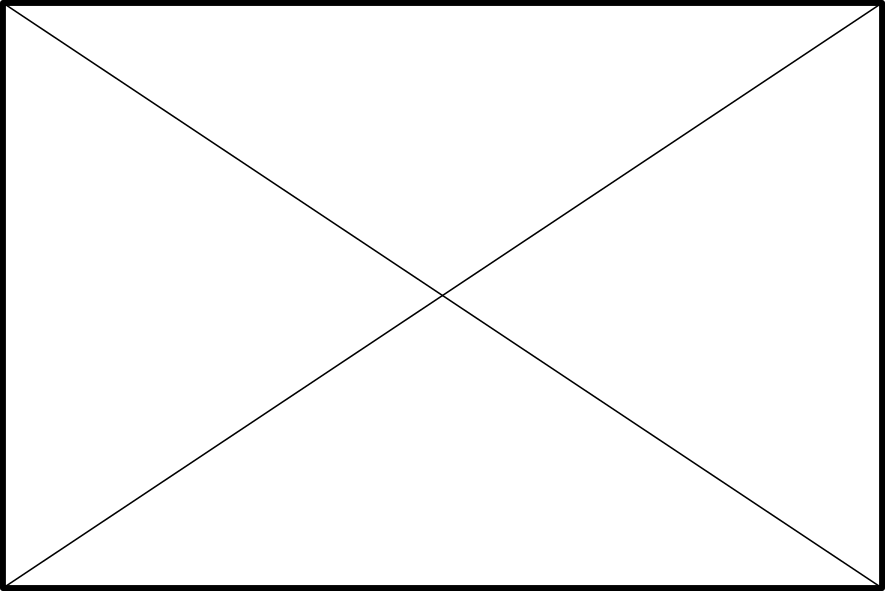
\includegraphics{TODO.png}
  \caption{Патч управления частотой радиостанции.}
  \label{patch:enc-count-freq}
\end{figure}

\section{Динамик}

% TODO: complete section

Извлечение звука — это физический процесс, при котором электрический ток должен проходить через катушку-магнит в динамике, которая в свою очередь то притягивает, то отталкивает мембрану. Мембрана толкает воздух с нужной частотой, а это уже и есть звук. В зависимости от того, насколько податливой окажется эта мембрана, источник аудиосигнала либо сможет её качать в эффективном дианазоне, либо нет.

\begin{figure}
  \centering
  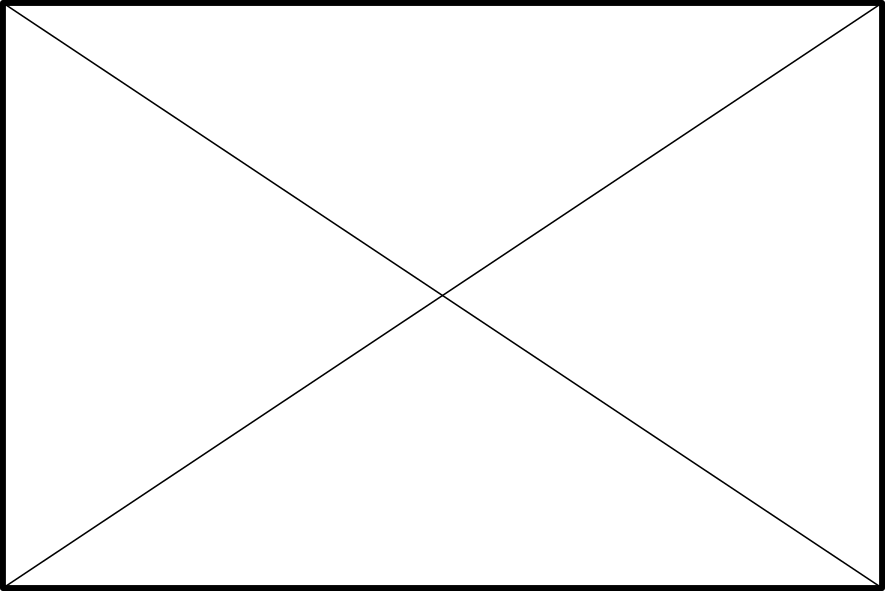
\includegraphics{TODO.png}
  \caption{Общий принцип извлечения звука.}
\end{figure}

Мерой этой податливости является \emph{импеданс}, характеристика динамиков, которая измеряется в омах. Для внешних ширпотребных динамиков типовым значением является 4--8 ом, для наушников — 24 и более ом. Чем импеданс ниже, тем легче качать мемрану, но при этом же, тем больше тока она потребляет. Если ток оказывается слишком большим, это может вывести из строя источник аудиосигнала.

\section{Звуковой усилитель}

Как я говорил ранее, выходной мощности одного лишь TEA5767 не хватит, чтобы выдавать звук на динамик приличного размера, а нам необходимо наполнить звуком хотя бы небольшую комнату.

Возможностей TEA5767 хватит лишь на извлечение тихого звука из небольших наушников. Предполагается, что после чипа будет стоять ещё один: \emph{усилитель звука}.\footnote{Англ. «Audio Amplifier».} Такая модульность вполне традиционна для мира микроэлектроники: один чип решает одну задачу и делает это хорошо. В конце концов, производитель FM-приёмника понятия не имеет динамики какой мощности захочет подключить к нему инженер-пользователь, а выпускать десятки моделей на все случаи жизни было бы коммерчески нецелесообразно. У нас внешний динамик, поэтому однозначно будем ставить звуковой усилитель.

\begin{Note}
  Да, существуют модули FM-приёмников, на которых уже установлен усилитель. Если у вас такой, изучите его характеристики и сопоставьте их с требованиями динамика. Если пасьянс сходится, можете пропустить следующий шаг. Если нет, ничего страшного: можно после интегрированного усилителя поставить дополнительный и более мощный внешний, и всё заработает.
\end{Note}

Аудио-усилитель — устройство на которое подают слабый аудиосигнал и питание, а на выходе получают кратно усиленный сигнал эквивалентной формы (рис. \ref{fig:sound-amp-diagram}). Получить сигнал идентичной формы не позволяют законы физики и битва между разными классами усилителей идёт за похожесть, а точнее за минимизацию искажений.

\begin{figure}
  \centering
  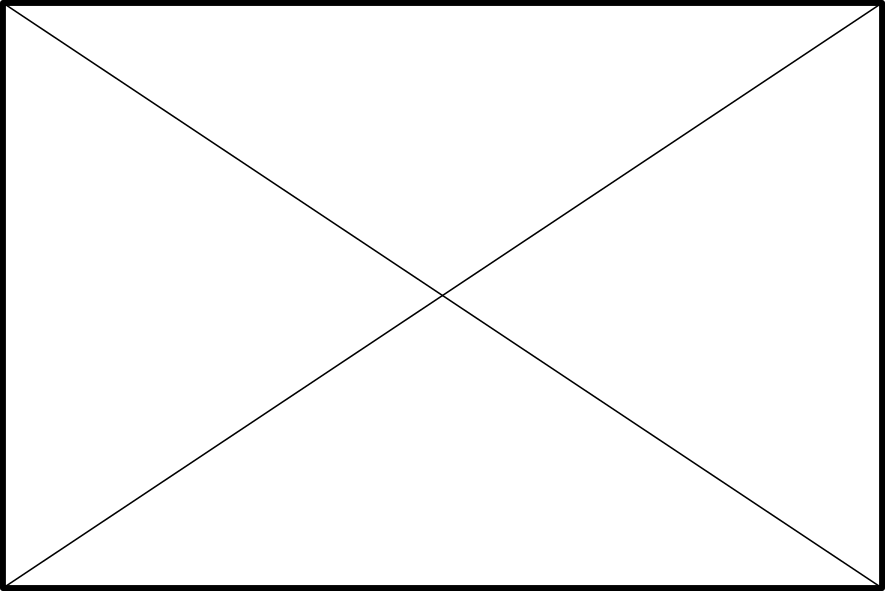
\includegraphics{TODO.png}
  \caption{Общий принцип работы звукового усилителя.}
  \label{fig:sound-amp-diagram}
\end{figure}

Нам понадобится микросхема-усилитель «класса D». К классу D относятся так называемые цифровые импульсные усилители. Они дешёвые, компактные и высокоэффективные: в нагрев уходит только 5-10\% энергии, остальное уходит в звук. Есть ещё другие классы: «A», «B», «AB», ламповые, но всё это настольные монстры-обогреватели (70\% — в нагрев) по цене чугунного моста для истинных аудиофилов. Большая часть потребительской электроники использует класс D.

\begin{figure}
  \centering
  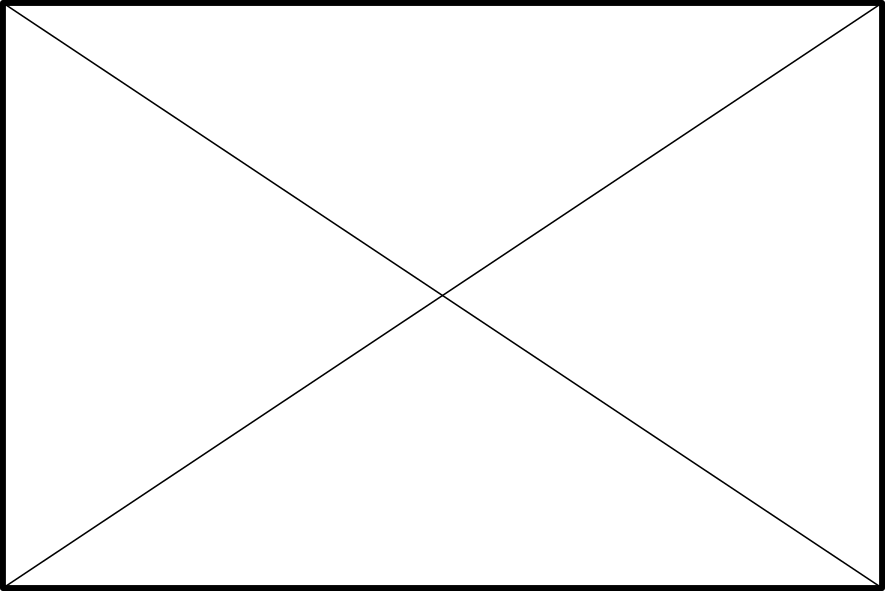
\includegraphics{TODO.png}
  \caption{Функциональная диаграмма устройства усилителя класса D.}
  \label{fig:sound-amp-class-d-diagram}
\end{figure}

Как обычно, удобнее будет воспользоваться готовым модулем нежели сырой микросхемой: на нём уже будет установлен необходимый обвес из конденсаторов, резисторов и дросселей. Я выбрал для проекта простой модуль на базе микросхемы усилителя PAM8403.

\begin{figure}
  \centering
  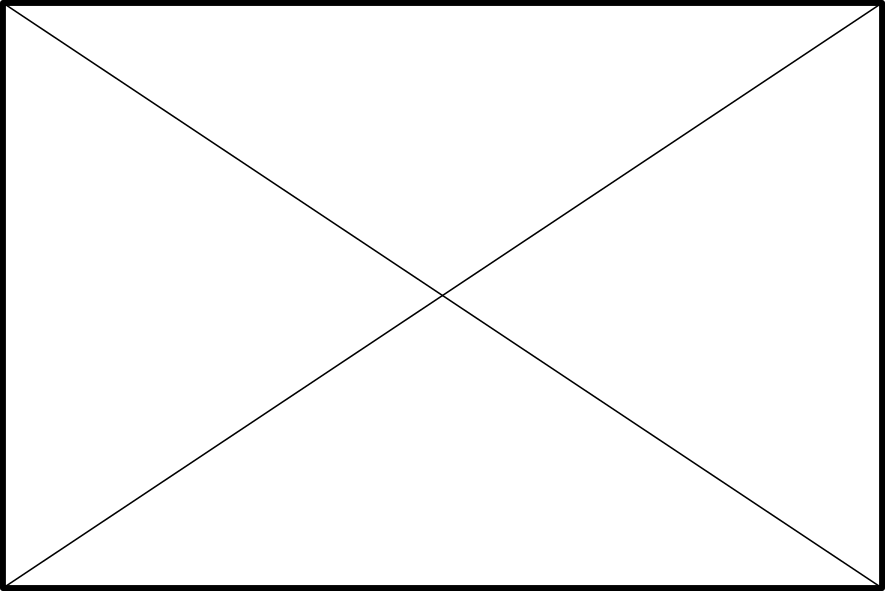
\includegraphics{TODO.png}
  \caption{Популярные модули на базе PAM8403.}
  \label{fig:pam8403-modules}
\end{figure}

\section{Управление громкостью}

А как управлять громкостью? Некоторые микросхемы-усилители являются управляемыми. В этом случае контроллер может говорить усилку громче/тише/цыц используя какой-нибудь интерфейс вроде I²C. Но в микросхеме PAM8403 такой функции попросту нет. На помощь снова приходят элементарные законы физики.

Чтобы сделать звучание тише, необходимо уменьшить ток протекающий через динамик. Ток в цепи уменьшает резистор. Помните, мы поставили такой между наушниками и выходом TEA5767 (рис. \ref{fig:tea5767-wiring})? Так вот, если так же поставить резистор между выходом усилителя и колонкой, её громкость снизится. И чем большим будет номинал резистора, тем тише будет звук. Мы хотим управлять громкостью налету, поэтому вместо постоянного резистора можно воспользоваться переменным. Как вы помните, переменный резистор также называют потенциометром.

\section{Потенциометр в роли резистора}

% TODO: complete section

\begin{figure}
  \centering
  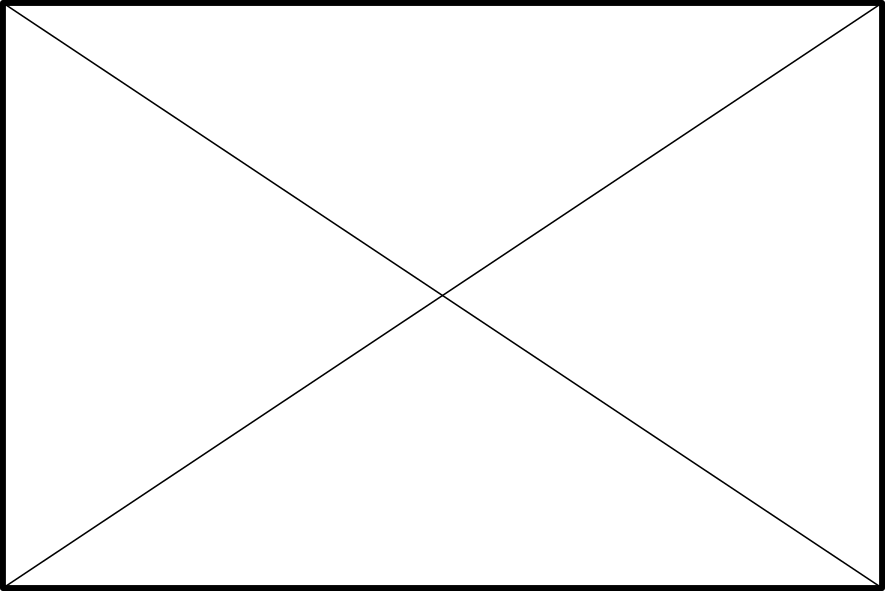
\includegraphics{TODO.png}
  \caption{Устройство потенциометра.}
  \label{fig:pot-internals}
\end{figure}

У переменного резистора три вывода. Между крайними выводами сопротивление всегда одинаково и равняется \emph{номинальному}, которое заявлено в его характеристиках, например: 10 килоом. Самое интересное происходит на центральном выводе, который подключен к бегунку.\footnote{Англ. «Washer»}. Сопротивление между ним и одним из крайних выводов меняется от нуля до номинала при повороте от одного предела до другого. Это то, что нам нужно: сигнал с усилителя мы можем подать на крайний вывод потенциометра, а центральный — отправить на динамик.

\begin{figure}
  \centering
  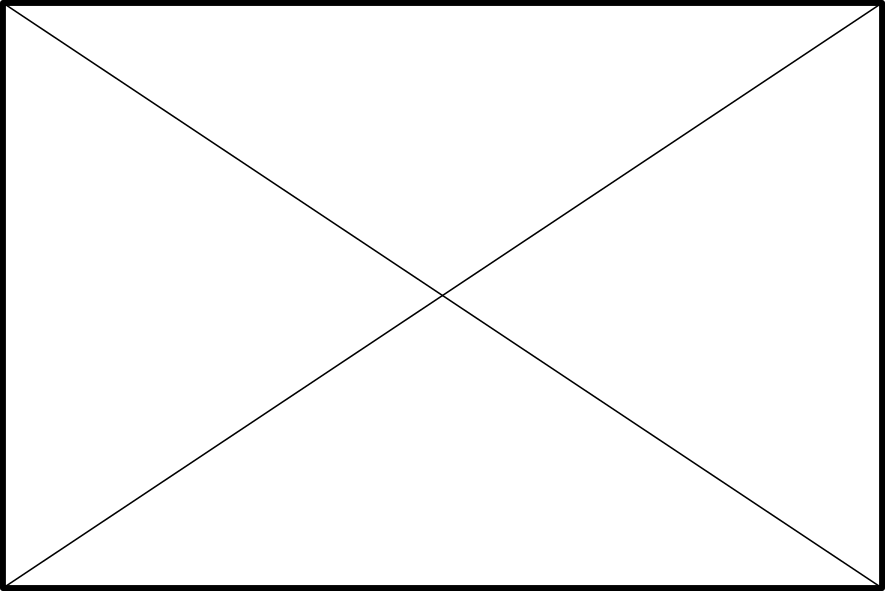
\includegraphics{TODO}
  \caption{Использование потенциометра для регулировки громкости.}
  \label{fig:pot-volume}
\end{figure}

В зависимости от того, какой из крайних выводов мы задействовали, громкость будет уменьшаться при повороте ручки по часовой или против часовой стрелки. Имейте это в виду, если регулировка громкости на вашем радио поведёт себя контринтуитивно.

\section{Меняем наушники на динамик}

Теперь, когда мы разобрались с необходимыми компонентами, пришло время дополнить наше устройство. Отключите устройство от питания, чтобы во время сборки нечаянно не закоротить чего-нибудь. Затем соберите схему, как показано на рисунке \ref{fig:amp-pot-speaker-wiring}. Скрестите пальцы и подавайте питание!

\begin{figure}
  \centering
  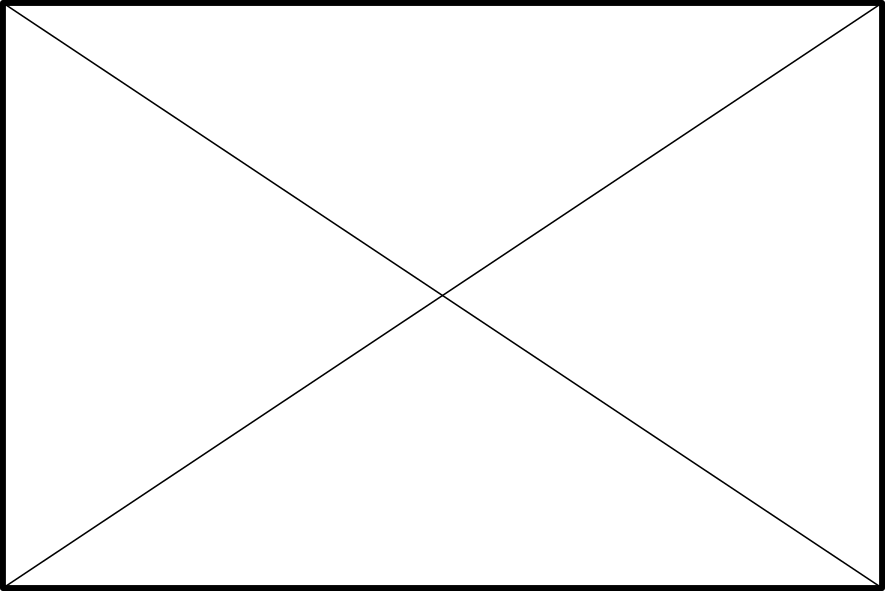
\includegraphics{TODO}
  \caption{Подключение аудио-усилителя, динамика и потенциометра регулировки громкости.}
  \label{fig:amp-pot-speaker-wiring}
\end{figure}

Обратите внимание, что конденсаторы и постоянные резисторы перед динамиком больше не нужны. Все функции защиты уже включены в модуль аудиоусилителя. Впрочем, если бы вы их оставили, всё продолжило бы работать.

Важный момент: динамик в нашем радио всего один, в отличие от наушников, где динамиков два. Поэтому мы подключаем только один из каналов. Стоит при этом перевести сам модуль FM-приёмника в режим «моно», чтобы качество звука не пострадало, если в трансляции встретятся эффекты, рассчитанные на стереозвучание.
В монофоническом режиме процессор FM-чипа усреднит сигнал левого и правого канала и выдаст одинаковый сигнал на оба. За эту настройку отвечает вход \texttt{STi} ноды \texttt{tea576x-fm-radio-i2c}. Чтобы перейти в моно-режим, выставьте его в \texttt{False} через панель инспектора. Перезалейте программу на контроллер и потестируйте как следует получившийся девайс.

Уже совсем похоже на то, что нужно. Осталось несколько штрихов.

\section{Текстовый экран}

\begin{figure}
  \centering
  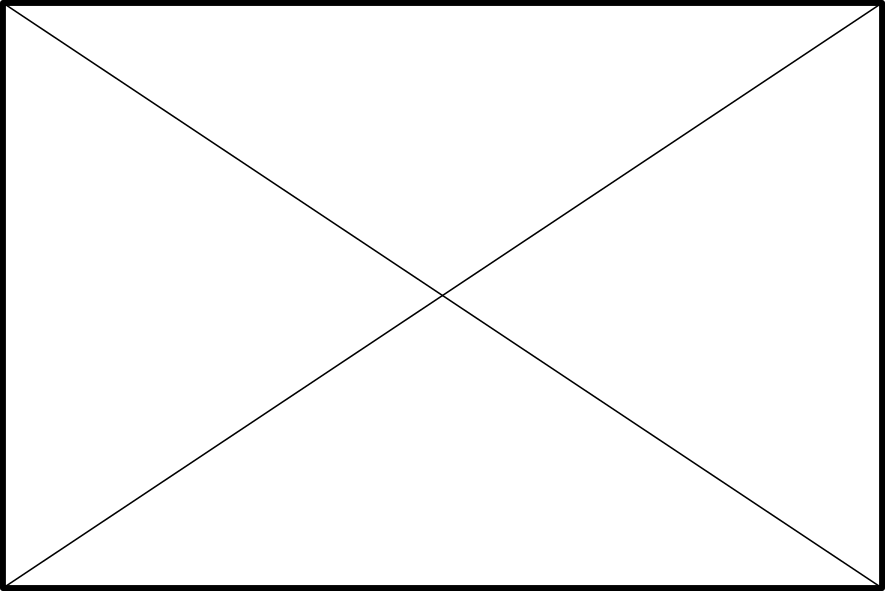
\includegraphics{TODO}
  \caption{Знакосинтезирующие дисплеи.}
\end{figure}

Было бы неплохо добавить к нашему радио индикацию. Без подключения к компьютеру, вслепую сложно найти нужную радиостанцию, даже если знаешь её частоту. Самое простое решение для вывода небольшого количества текста и чисел — знакосинтезирующий дисплей.\footnote{Англ. «Text Display» или «Text LCD». Он же текстовый экран, он же текстовый ЖК-дисплей. Иногда встречаются такие дисплеи на технологии OLED, сути не меняет, но называют их «текстовый OLED»} Они не могут показывать произвольную графику, но отлично справляются с выводом монохромного текста. Вы наверняка встречались с такими дисплеями на вендинговых автоматах или кофе-машинах.

Экран дисплея разделён на прямоугольные знакоместа. Каждое из них состоит из сетки 5×8 символов. В каждом из знакомест можно вывести один из символов, который прошит производителем в памяти дисплейного модуля, в так называемой кодовой таблице (рис. \ref{fig:text-lcd-code-page}). Несколько символов в кодовой таблице, как правило, доступны для изменения пользователем, чтобы можно было создать иконки специально для своего проекта.

\begin{figure}
  \centering
  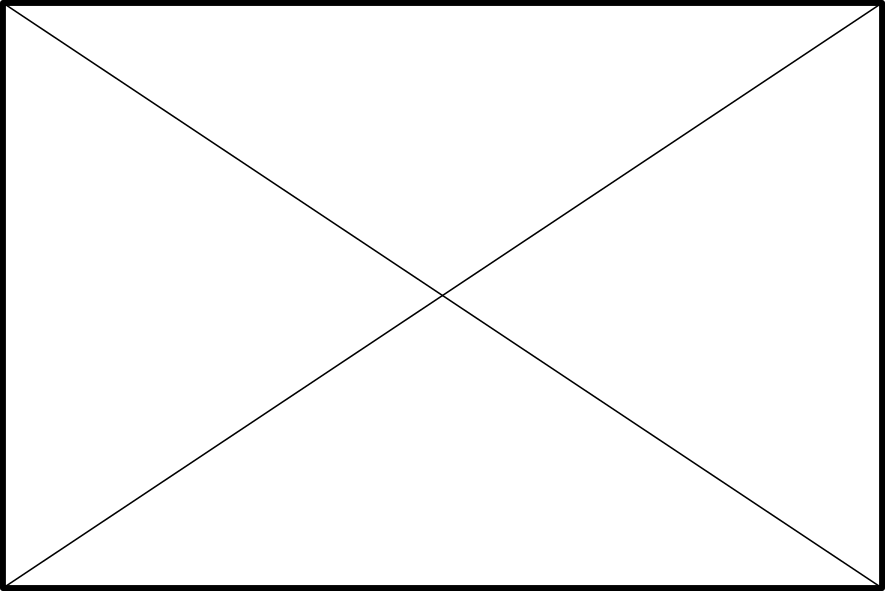
\includegraphics{TODO}
  \caption{Принцип вывода информации на текстовый дисплей.}
\end{figure}

\begin{figure}
  \centering
  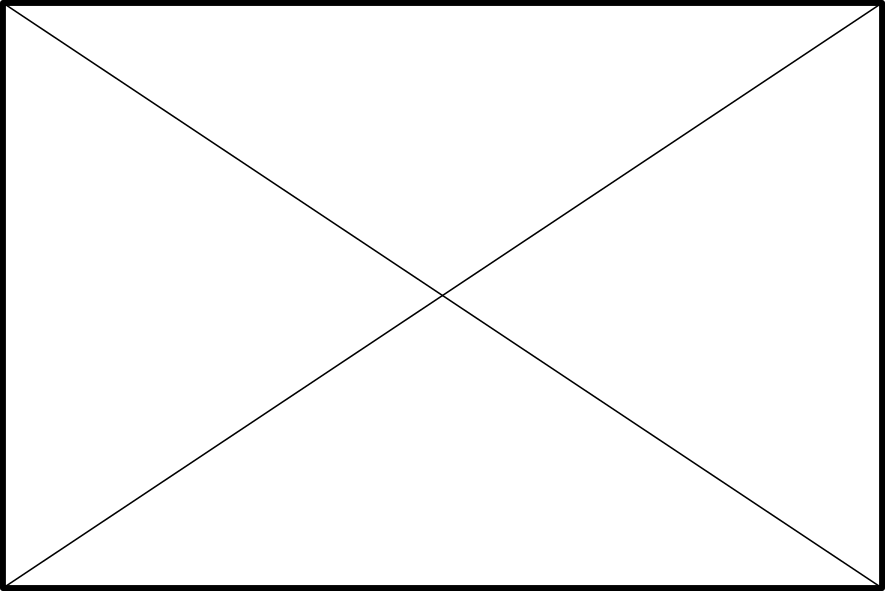
\includegraphics{TODO}
  \caption{Пример кодовой таблицы дисплея. В данном случае от компании МЭЛТ.}
  \label{fig:text-lcd-code-page}
\end{figure}

Текстовые дисплеи различаются по характеристикам:

\begin{itemize}
  \item количество знакомест: самые популярные — 16×2 (16 символов в строке, 2 строки), 20×4, 8×2;
  \item физический размер экрана;
  \item цвет подсветки;
  \item локализация таблицы символов: какой алфавит помимо латинского можно вывести;
  \item инерфейс подключения: параллельный или I²C.
\end{itemize}

Дисплеи корректнее называть дисплейными модулями ведь они состоят из экрана, микросхемы-процессора (драйвера), чипа энергонезависимой памяти и компонентов обвязки. Исторически самой популярной миркросхемой-процессором стала HD44780 от Hitachi. Подавляющее большинство таких дисплеев выпускают или на этом драйвере, или на один-в-один совместимом. Это и определило традиционнй интерфейс подключения экрана: \emph{параллельный}. В параллельном интерфейсе, в отличии от последовательного, биты передаются по проводам не один за другим, а сразу группами по 4 или 8 штук за такт. Это увеличивает скорость коммуникации, но требует для подключения сразу 6-8-10 проводов и пинов вашего контроллера (рис. \ref{fig:text-lcd-parallel-8}).

\begin{figure}
  \centering
  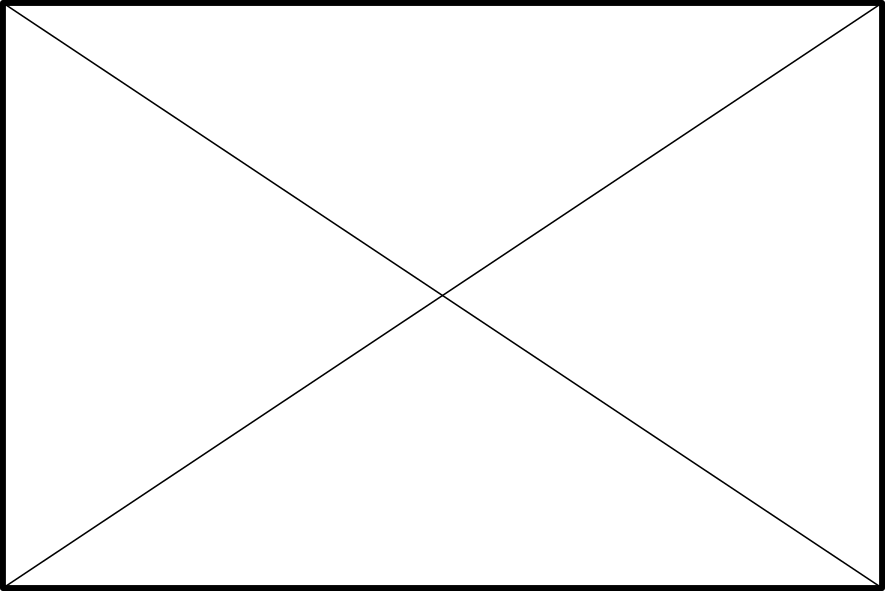
\includegraphics{TODO}
  \caption{Подключение дисплея с параллельным интерфесом по полной.}
  \label{fig:text-lcd-parallel-8}
\end{figure}

\begin{Note}
  Более высокая скорость передачи в параллельном интерфейсе — это уже миф. Из-за того, что электромагнитные наводки линий друг на друга мешали до бесконечности увеличивать скорость, в какой-то момент времени разные инженерные трюки позволили сделать последовательные интерфесы гораздо более скоростными. Недаром одним из самых распространённых скоростных интерфейсов стал USB: Universal \textbf{Serial} Bus (универсальная \textbf{последовательная} шина).
\end{Note}

Именно параллельным интерфейсом обусловлена гребёнка внушительных размеров для подключения экрана. Можно встретить 16 и 20-пиновые модели дисплеев. На практике не обязательно подключать все. В четырёхбитном режиме от контроллера понадобится «всего» 6 пинов, пара проводов для питания драйвера и пара для включения подсветки (рис. \ref{fig:text-lcd-parallel-4}). Как ни крути, это всё равно много и не практично. Поэтому, всевышний, благослови того человека, который придумал установить на входе драйвера дисплея \emph{I²C-расширитель портов}. Благодаря этому дополнительному чипу на плате дисплейного модуля его внутреннее устройство остаётся неизменным, а с точки зрения внешнего мира, то есть контроллера, дисплей становится простым I²C-модулем с возможностью управления по двум линиям (см. раздел «\nameref{I2C}»). На таких моделях дисплеев обычно требуется лишь одна пара проводов питания, которое одновременно используется и драйвером, и подсветкой. Бонус: управлять подсветкой становится возможным программно, с помощью специальной команды I²C.

\begin{figure}
  \centering
  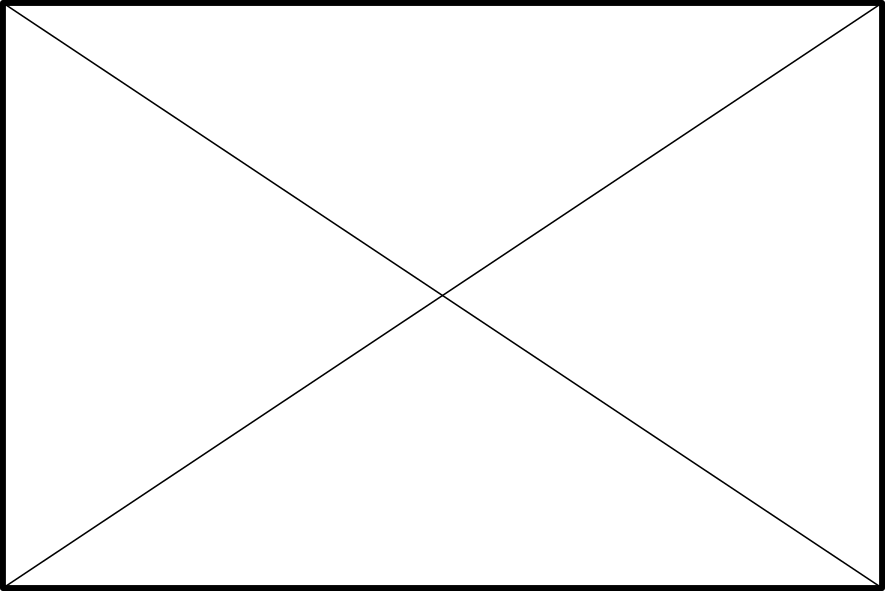
\includegraphics{TODO}
  \caption{Подключение дисплея с параллельным интерфесом в четырёхбитном режиме.}
  \label{fig:text-lcd-parallel-4}
\end{figure}

\begin{figure}
  \centering
  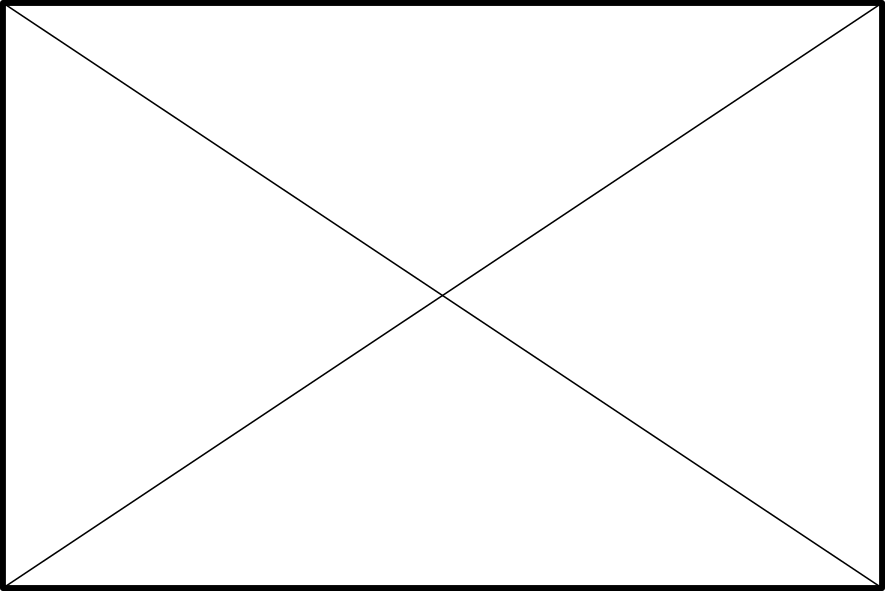
\includegraphics{TODO}
  \caption{Подключение дисплея с интерфейсом I²C.}
  \label{fig:text-lcd-i2c}
\end{figure}

Для собственных Arduino-проектов, я рекомендую выбирать именно дисплеи с поддержкой I²C. У некоторых из них наружу выведены только 4 необходимых пина для подключения, другие являются гибридами. На гибридах выведены все контакты, а вы сами решаете в каком режиме будете использовать дисплей: параллельном или I²C.

\section{Подключаем экран к радио}

Для нашего устройства я выбрал экран размером 16×2 с интерфейсом I²C и янтарной подсветкой. Как вы помните, у нас на шине I²C уже находится модуль FM-приёмника TEA5767, но это дисплею не помеха. Напротив, перед нами открывается вся прелесть шины: сигнальных линий по-прежнему две, а устройств уже несколько. Различать их контроллер сможет благодаря тому, что у них разные адреса: 60h у FM-приёмника и 38h у дисплея.

Отключите питание. Подключите дисплей, как показано на рисунке \ref{fig:text-lcd-radio-wiring}. Подключайте USB снова и приступаем к программированию!

\begin{figure}
  \centering
  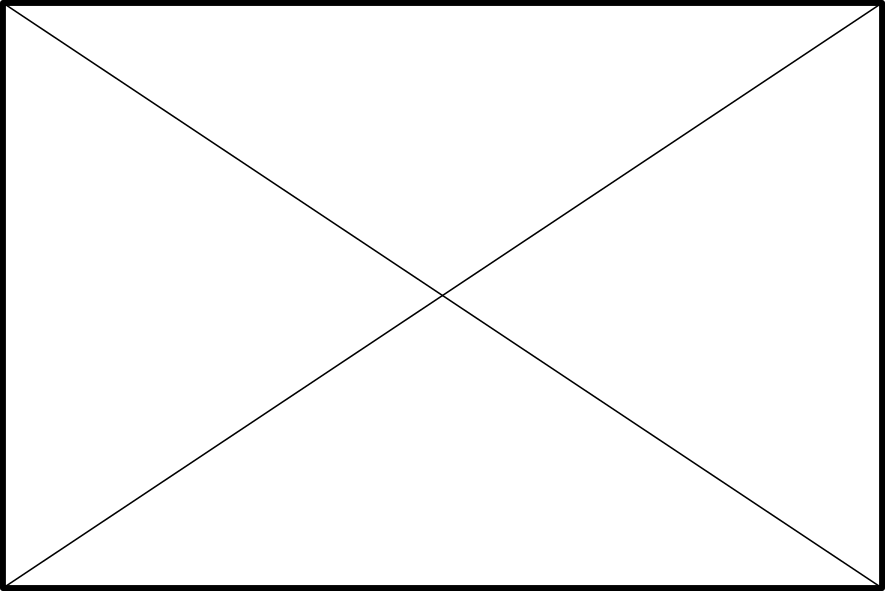
\includegraphics{TODO}
  \caption{Схема подключения экрана на шину, рядом с FM-модулем.}
  \label{fig:text-lcd-radio-wiring}
\end{figure}

\section{Нода text-lcd-16x2-i2c}

Мы хотим выводить на экран текущую выбранную частоту радио. Давайте сделаем это на первой строке экрана.

Для управления нашим текстовым экраном в XOD уже есть быстро-нода в стандартной библиотеке \texttt{xod-dev/text-lcd}. Она называется, вы догадались, \texttt{text-lcd-16x2-i2c}. Добавьте её на патч с радио и рассмотрите входы.

\begin{figure}
  \centering
  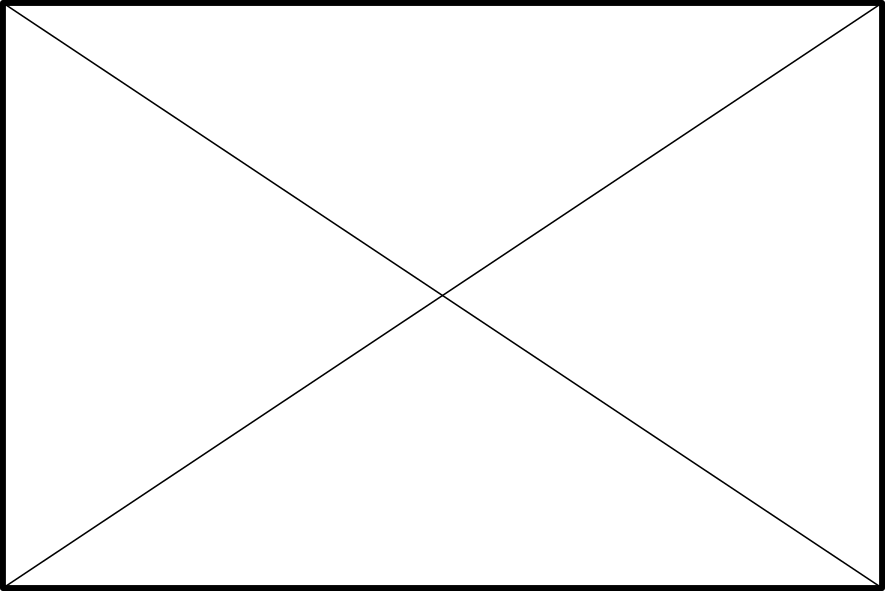
\includegraphics{TODO}
  \caption{Нода text-lcd-16x2-i2c}
\end{figure}

\begin{itemize}
  \item \texttt{ADDR} — I²C адрес экрана. В моём случае нужно выставить \texttt{38h}. Обратитесь к спецификации от производителя, чтобы узнать адрес своего дисплея.
  \item \texttt{BL} управляет подсветкой экрана: \texttt{True} — включена, \texttt{False} — выключена.
  \item \texttt{L1}/\texttt{L2} задаёт текст на первой и второй строке соответственно.
\end{itemize}

Пока что оставим вторую строку в покое, а на первую выведем значение текущей частоты. Нода \texttt{watch} нам больше не понадобится. И вместо того, чтобы выводить значение на неё, отправьте его на вход \texttt{L1} ноды-дисплея (рис. \ref{patch:lcd-freq}). Загружайте программу на котроллер и крутите ручку! Дисплей отображает текущую частоту. Прекрасно! Не правда ли?

\begin{figure}
  \centering
  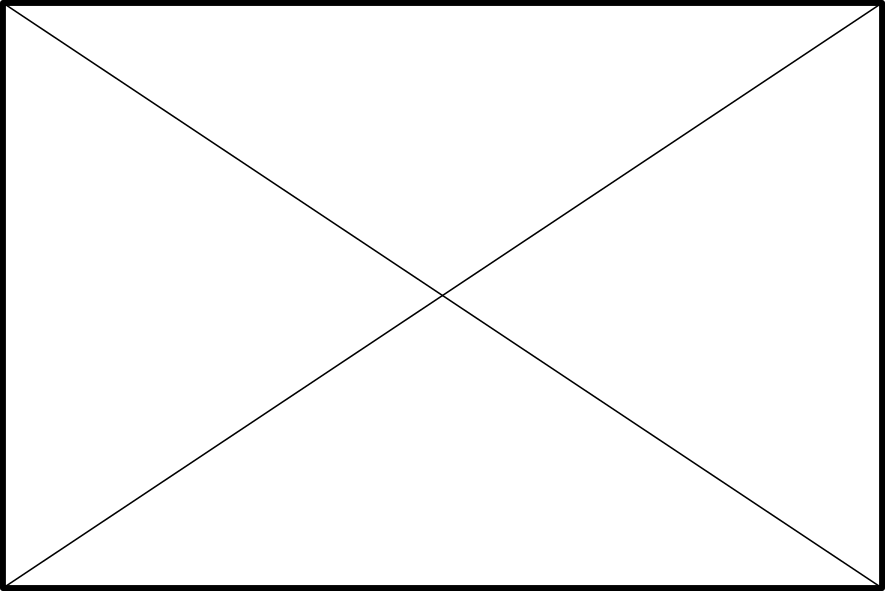
\includegraphics{TODO}
  \caption{Патч радио с выводом частоты на экран.}
  \label{patch:lcd-freq}
\end{figure}

Окей, с точки зрения эстета одинокое «89.50» на первой строке выглядит не очень внятно: на конце явно лишний нолик, не сразу очевидно, что это число показывает. Сделаем вывод более понятным при помощи пары нод, связанных с форматированием текста.

\section{Выводим станцию на дисплей используя текстовые ноды}

Давайте сначала сформулируем цель: как должен выглядеть «правильный» вывод радиостанции на экран. Допустим, так:

\begin{itemize}
  \item \makebox[40pt][l]{Было:} \lcd{98.5\ \ \ \ \ \ \ \ \ \ \ \ }
  \item \makebox[40pt][l]{Станет:} \lcd{FM\ 98.5\ MHz\ ***\ }
\end{itemize}

Звёздочками будем выводить уровень качества сигнала: одна — это грусть, три — это супер.

Для начала избавимся от лишнего нолика. По умолчанию в XOD числа при автоматическом преобразовании в строку форматируются с точностью до двух знаков дробной части. Нам с нашим радио нужен всего один. Изменить точность позволяет нода \texttt{format-number} из стандартной библиотеки \texttt{xod/text}. У неё есть вход \texttt{DIG}, который определяет количество знаков дробной части. Поставьте такую ноду в разрыв между нодой счётчика и дисплея, выставив значение \texttt{DIG} в \texttt{1} (рис. \ref{patch:fm-format-number}).

\begin{figure}
  \centering
  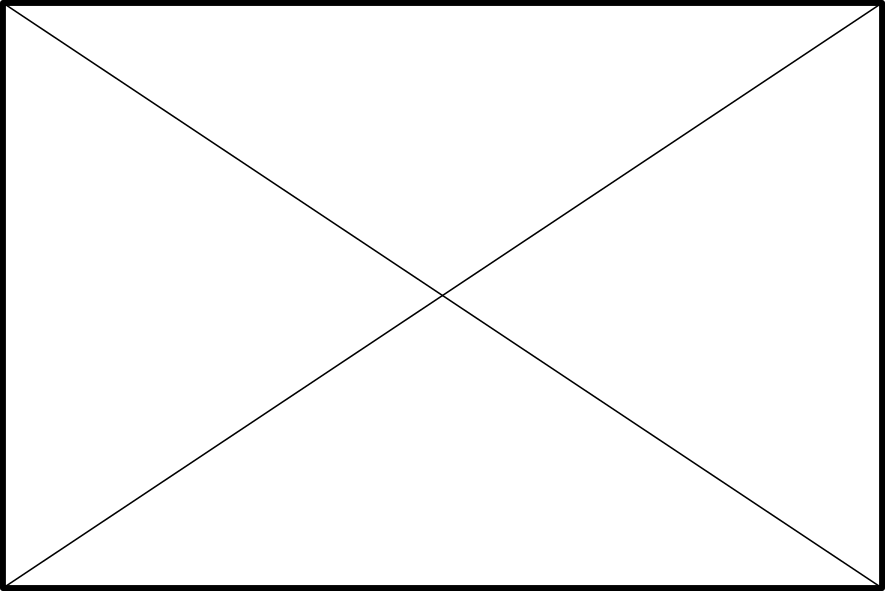
\includegraphics{TODO}
  \caption{Патч с округлением частоты до одного знака.}
  \label{patch:fm-format-number}
\end{figure}

Загружайте программу и смотрите за результатом. Нолик исчез, уже неплохо!

Теперь нужно добавить префикс «FM» и суффикс «MHz» к нашей строке. За склейку строки из нескольких кусочков отвечает нода \texttt{xod/text/join}. Добавьте её на патч, в разрыв между \texttt{format-number} и нодой дисплея. Первый вход, \texttt{D} определяет разделитель между кусочками. По умолчанию это пробел: то, что нужно, оставьте. Входу \texttt{S1} назначьте значение \texttt{"FM"}, на вход \texttt{S2} отправьте результат \texttt{format-number}, а на \texttt{S3} — \texttt{"MHz"}. Стоп, а третьего входа для строки нет! Это вы его не видите, а он есть. Нода \texttt{join} относится к так называемым \emph{вариадичным}\footnote{Англ. «Variadic»} нодам. Вариадичным нодам можно неограничено добавлять количество входных пинов. Для этого потяните за выступ справа: появится ещё один пин. К нему-то и привяжите значение \texttt{"MHz"} (рис. \ref{patch:fm-join}).

\begin{figure}
  \centering
  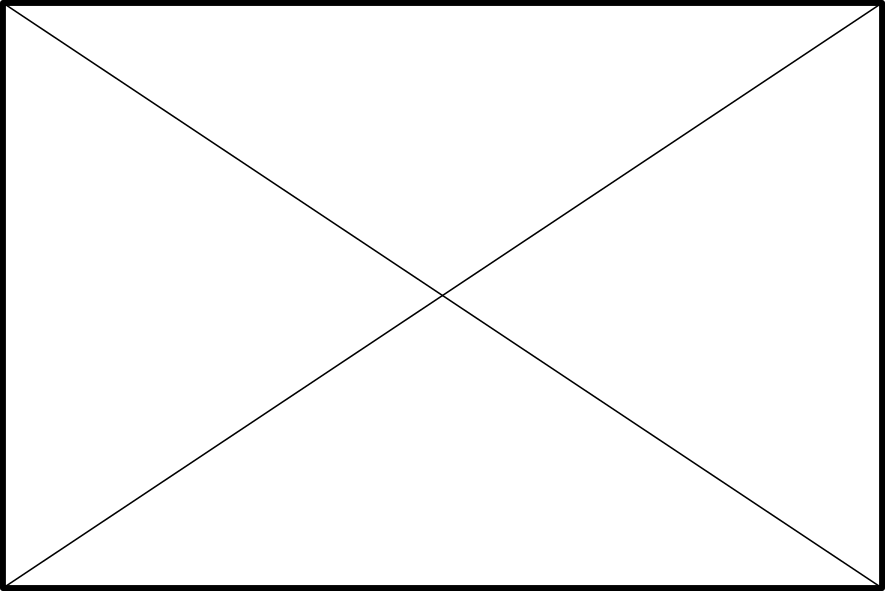
\includegraphics{TODO}
  \caption{Патч с префиксом и суффиксом вокруг частоты.}
  \label{patch:fm-join}
\end{figure}

Загружайте, смотрите, что получилось. Всё работает? Отлично!

Теперь к уровню сигнала. Нода \texttt{tea576x-fm-radio-i2c} выдаёт его в диапазоне от 0.0 до 1.0. А нам нужны от одной до трёх звёздочек. Спроецировать значение из одного диапазона на другой поможет нода \texttt{map-01-to} из \texttt{xod/math} (рис. \ref{patch:node-map-01-to}). Она принимает границы целевого диапазона \texttt{Tmin}/\texttt{Tmax} и само значение \texttt{X}. Воспользуемся ей, чтобы отобразить исходный диапазон [0; 1] в нужный нам [1; 3].

\begin{figure}
  \centering
  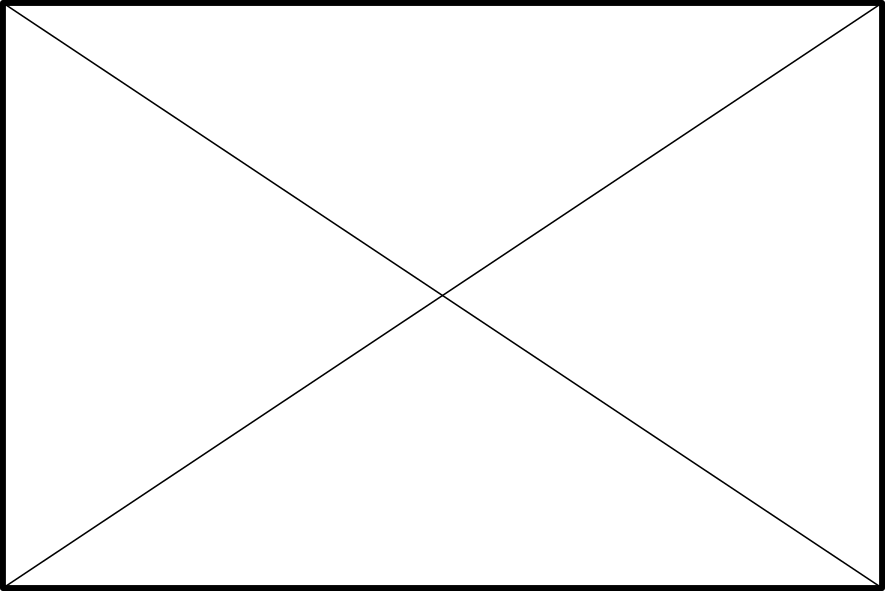
\includegraphics{TODO}
  \caption{Нода map-01-to.}
  \label{patch:node-map-01-to}
\end{figure}

Но нам ведь нужно даже не число от 1 до 3, а строка с таким количеством звёздочек. Для этого подойдёт нода \texttt{xod/text/repeat} (рис. \ref{patch:node-repeat}). Она принимает строку \texttt{S}, которую нужно повторять и количество повторений \texttt{N}. В качестве \texttt{S} используем звёздочку \texttt{"*"}, а на \texttt{N} заведём значение полученное из \texttt{node-map-01-to}.

\begin{figure}
  \centering
  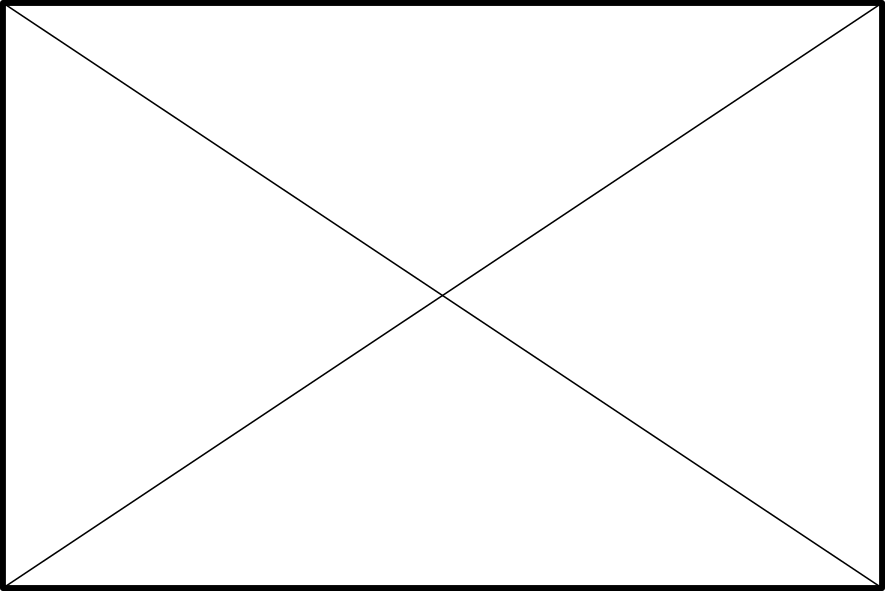
\includegraphics{TODO}
  \caption{Нода repeat.}
  \label{patch:node-repeat}
\end{figure}

И наконец, результат мы добавим через ноду \texttt{join} в конец строки. Собирая всё воедино, получаем патч, как на рисунке \ref{patch:fm-lcd-line-1}.

\begin{figure}
  \centering
  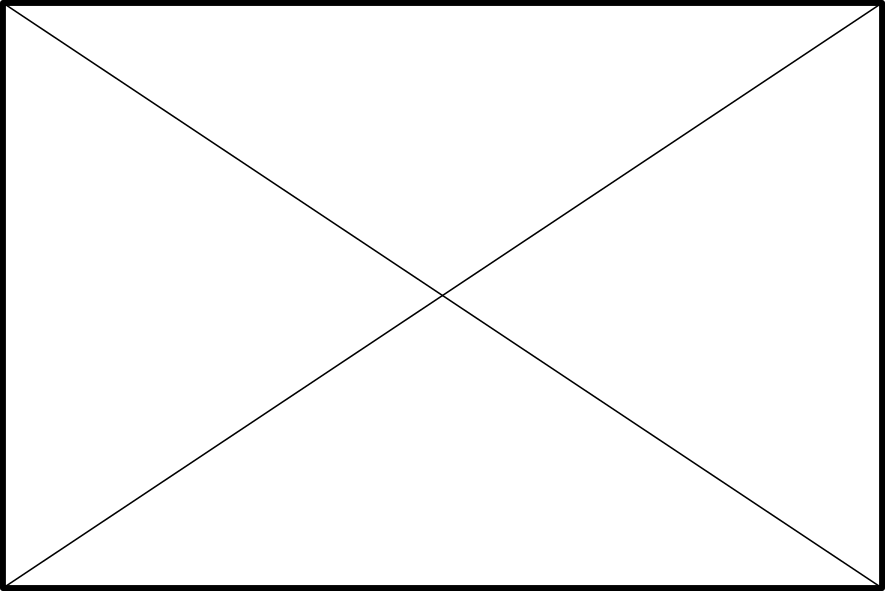
\includegraphics{TODO}
  \caption{Патч радио с выводом информации о текущей радиоволне.}
  \label{patch:fm-lcd-line-1}
\end{figure}

Загружаем, проверяем! Функциональная часть радио готова! И можно было бы уже переходить к корпусированию, но мы ведь перфекционисты? Регулировка громкости оторвана от устройства... Было бы замечательно подружить её с экраном.

%\section{Потенциометр в роли сенсора}
%\section{Вывод громкости на экран}
%\section{Добавляем аккумулятор}
%\section{Помещаем в корпус}
